\documentclass[12pt]{article}

\usepackage[margin=1in]{geometry} 
\usepackage{amsmath,amsthm,amssymb}
\usepackage{graphicx}
\usepackage{bm}
\usepackage[normalem,normalbf]{ulem}

\usepackage{tikz}
\newcommand*\circled[1]{\tikz[baseline=(char.base)]{
		\node[shape=circle,draw,inner sep=2pt] (char) {#1};}}

\newcommand{\N}{\mathbb{N}}
\newcommand{\Z}{\mathbb{Z}}

\DeclareMathOperator{\lcm}{lcm}

\newtheorem{theorem}{Theorem}

\newenvironment{exercise}[2][Exercise]{\begin{trivlist}
		\item[\hskip \labelsep {\bfseries #1}\hskip \labelsep {\bfseries #2.}]}{\end{trivlist}}

\makeatletter
\renewcommand*\env@matrix[1][*\c@MaxMatrixCols c]{%
	\hskip -\arraycolsep
	\let\@ifnextchar\new@ifnextchar
	\array{#1}}
\makeatother



\begin{document}
	
	% --------------------------------------------------------------
	%                         Start here
	% --------------------------------------------------------------
	
	
	\title{Homework 12 (Due Nov 14, 2022)}
	\author{Jack Hyatt\\ %replace with your name
		MATH 574 - Discrete Mathamatics - Fall 2022} 
	
	\maketitle
	
	Justify all of your answers completely.\\
	
	\renewcommand{\qedsymbol}{$\blacksquare$}
	
	\medskip 



\begin{enumerate}
\item Let $m,n,c \in \mathbb Z$. Prove that if $c \mid m$ and $c \mid n$ then $c \mid \gcd(m,n)$. 
\begin{proof}
	Let $m,n,c \in \mathbb Z$. Assume $c \mid m$ and $c \mid n$.\\
	So $\exists a,b\in\Z$ s.t. $ac = m$ and $bc=n$. \\
	B\'ezout's identity says that $\exists s,t\in\Z$ s.t. $sm+tn = \gcd(m,n)$.\\
	So $sm+tn = \gcd(m,n) \implies s(ac)+t(bc) = \gcd(m,n) \implies c(sa+tb) = \gcd(m,n)$. So c $\mid \gcd(m,n)$.
\end{proof}

\medskip

\item For nonzero integers $m,n, \ell \in \mathbb Z$ let $\gcd(m,n,\ell)$ denote the largest positive integer that divides all of $m, n,$ and $\ell$. Prove that $\gcd(m,n,\ell) = \gcd(\gcd(m,n), \ell)$. 
\begin{proof}
	Let $m,n, \ell \in \mathbb Z$ be nonzero. Set $k = \gcd(m,n,\ell)$. So $k \leq \gcd(m,n)$ too by how gcd is defined for more than 2 inputs.\\
	So $k \mid m$, $k \mid n$, and $k \mid \ell$. So then $k \mid \gcd(m,n)$ by (1).
	So $k \mid \gcd(\gcd(m,n),\ell)$.\\
	Assume for contradiction that $\exists h\in\Z$ s.t. $h>k$ and $h=\gcd(\gcd(m,n),\ell).$\\
	So h divides both $\gcd(m,n)$ and $\ell$. Since divides is a transitive relation, h also divides m and n. So h divides all m,n and $\ell$. So since $h>k$ and divides all three, it should be the $\gcd(m,n,\ell)$. But we defined k as the $\gcd(m,n,\ell)$. So therefore, k must also be the $\gcd(\gcd(m,n),\ell)$.
\end{proof}


\medskip

\item Use the previous problem to prove that for nonzero integers $m, n, \ell \in \mathbb Z$, there exists integers $a,b,c \in \mathbb Z$ such that $am + bn + c\ell = \gcd(m,n,\ell)$.
\begin{proof}
	Redefine $\gcd(m,n,\ell)$ as $\gcd(\gcd(m,n),\ell)$ using (2). So using B\'ezout's identity, we get that $\gcd(\gcd(m,n),\ell) = s\cdot\gcd(m,n)+t\ell$ for some integers s,t. Using the identity again, we get $s\cdot\gcd(m,n)+t\ell = s(am+bn) + t\ell$ for some integers a,b.\\
	So $\gcd(m,n,\ell) = sam + sbn + t\ell$.
\end{proof}

\medskip

\item Alice has RSA public key $(13, 85)$. You intercept the encrypted message ``39" which was sent to Alice from Bob. Decrypt the message to obtain the plaintext message that Bob sent.  You may use a calculator.\\

So we'll have the expression $39\equiv m^{13}\mod 85$. So since $85 = 5\cdot17$, we get that $\phi(85) = 4\cdot16 = 64$. So now we need to choose a $d$ s.t. $13d\equiv1\mod64$. $d=5$ works. So now all we need to do is compute $39^5\mod85$, which is 14.

\medskip

\item For a positive integer $k$, we say a graph $G$ is $k$-regular if every vertex in $G$ has degree $k$. 
\begin{enumerate}
\item Draw a graph on 6 vertices that is 1-regular.\\
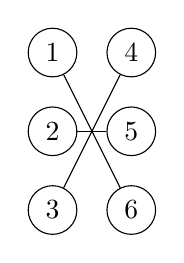
\begin{tikzpicture}[main/.style = {draw, circle}]
	\node[main] (1) {1};
	\node[main] (2) [below of=1] {2};
	\node[main] (3) [below of=2] {3};
	\node[main] (4) [right of=1] {4};
	\node[main] (5) [below of=4] {5};
	\node[main] (6) [below of=5] {6};
	\draw (1) -- (6);
	\draw (2) -- (5);
	\draw (3) -- (4);
\end{tikzpicture}
\item Draw two distinct graphs on 6 vertices that are 2-regular.
{\em Here distinct means non-isomorphic.}\\
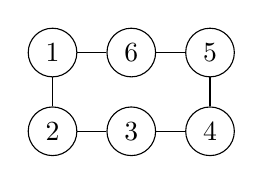
\begin{tikzpicture}[main/.style = {draw, circle}]
	\node[main] (1) {1};
	\node[main] (2) [below of=1] {2};
	\node[main] (3) [right of=2] {3};
	\node[main] (4) [right of=3] {4};
	\node[main] (5) [above of=4] {5};
	\node[main] (6) [left of=5] {6};
	\draw (1) -- (6);
	\draw (1) -- (2);
	\draw (2) -- (3);
	\draw (3) -- (4);
	\draw (4) -- (5);
	\draw (6) -- (5);
\end{tikzpicture}\\\\
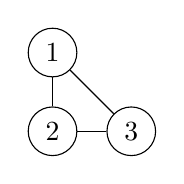
\begin{tikzpicture}[main/.style = {draw, circle}]
	\node[main] (1) {1};
	\node[main] (2) [below of=1] {2};
	\node[main] (3) [right of=2] {3};
	\draw (1) -- (2);
	\draw (2) -- (3);
	\draw (1) -- (3);
\end{tikzpicture}
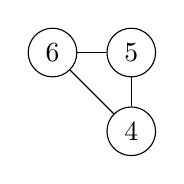
\begin{tikzpicture}[main/.style = {draw, circle}]
	\node[main] (4) {4};
	\node[main] (5) [above of=4] {5};
	\node[main] (6) [left of=5] {6};
	\draw (4) -- (5);
	\draw (4) -- (6);
	\draw (6) -- (5);
\end{tikzpicture}

\item Draw two distinct graphs on 6 vertices that are 3-regular.\\
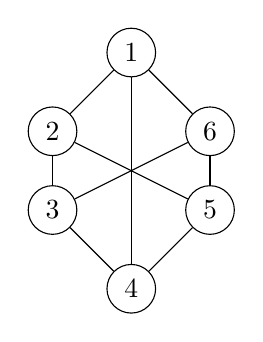
\begin{tikzpicture}[main/.style = {draw, circle}]
	\node[main] (1) {1};
	\node[main] (2) [below of=1,left of=1] {2};
	\node[main] (3) [below of=2] {3};
	\node[main] (4) [below of=3,right of=3] {4};
	\node[main] (5) [above of=4, right of=4] {5};
	\node[main] (6) [above of=5] {6};
	\draw (1) -- (6);
	\draw (1) -- (2);
	\draw (2) -- (3);
	\draw (3) -- (4);
	\draw (4) -- (5);
	\draw (6) -- (5);
	\draw (1) -- (4);
	\draw (3) -- (6);
	\draw (2) -- (5);
\end{tikzpicture}\\\\
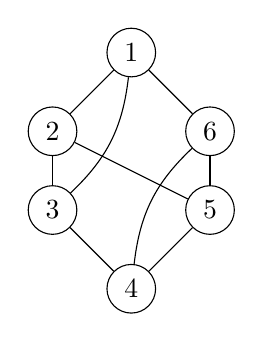
\begin{tikzpicture}[main/.style = {draw, circle}]
	\node[main] (1) {1};
	\node[main] (2) [below of=1,left of=1] {2};
	\node[main] (3) [below of=2] {3};
	\node[main] (4) [below of=3,right of=3] {4};
	\node[main] (5) [above of=4, right of=4] {5};
	\node[main] (6) [above of=5] {6};
	\draw (1) -- (6);
	\draw (1) -- (2);
	\draw (2) -- (3);
	\draw (3) -- (4);
	\draw (4) -- (5);
	\draw (6) -- (5);
	\draw[bend left=20] (1) to (3);
	\draw[bend left=20] (4) to (6);
	\draw (2) -- (5);
\end{tikzpicture}\\\\
\item Prove that if $k$ is odd, then there cannot exist a $k$-regular graph with an odd number of vertices.
\begin{proof}
The handshaking lemma states that summing up all the degree's of the nodes will be twice the amount of edges, an even number. If we were to have odd number of nodes, each with an odd degree $k$, summing them up would give us an odd number multiplied by an odd number, which is odd. But Handshaking lemma says it needs to be even, a contradiction. So there cannot both be an odd number of nodes in an odd $k$-regular graph.
\end{proof}
\end{enumerate}

\medskip

\item Let $G$ be a bipartite graph with bipartition $X \cup Y$. Prove that if $G$ is $k$-regular for some $k \in \mathbb N$, then $|X| =|Y|$. 
\begin{proof}
	Assume G is a regular bipartite graph with degree k. Let X and Y be the two partitions of the bipartite graph.\\
	Since G bipartite, $E(X)=E(Y)$. Since G is regular $E(X) = k|X|$, and $E(Y)=k|Y|$. So $E(X)=E(Y) \implies k|X|=k|Y| \implies |X|=|Y|$.  So G is a balanced bipartite graph.\\
\end{proof}

\medskip


\item Prove or disprove the following statements.
\begin{enumerate}
\item If $G$ is an $n$-vertex graph in which every vertex has degree at least $\lceil (n-1)/2 \rceil$, then $G$ is connected.
\begin{proof}
	Let G be an $n$-vertex graph in which every vertex has degree at least $\lceil (n-1)/2 \rceil$. Assume towards contradiction that $G$ is not connected. So then $G$ has at least 2 connected components.\\
	WLOG, let A be the connect component with the least number of vertices. Since there are at least two connect components, the most amount of vertices in A can be $\lfloor (n-1)/2 \rfloor$. Looking at a vertex, $v$, in A, the most edges it can have can be $\lfloor (n-1)/2 \rfloor-1$. But every vertex in G must have degree at least $\lceil (n-1)/2 \rceil$, which is strictly larger than what $v$ is allowed, a contradiction.
\end{proof}

\item If $G$ is an $n$-vertex graph in which every vertex has degree at least $\lfloor (n-2)/2 \rfloor$, then $G$ is connected.\\\\
This is easily disproved by considering the graph with just 2 nodes and no edges. Each node will clearly have at least degree $\lfloor (2-2)/2 \rfloor$, or just 0, and the graph is not connected.
\end{enumerate}

\medskip 

\item Suppose that $G$ is a graph with in which every vertex has degree at least $k \geq 2$. 
\begin{enumerate}
\item Prove that $G$ contains a cycle with at least $k+1$ vertices.\\
\begin{proof}
	Let $P=v_0\ldots v_n$ be the longest path in G. So then the neighborhood of $v_0$ must be in the path, because otherwise the path would be longer. So let the neighbor of $v_0$ with the highest index in the path be $v_\ell$. Since $v_0$ must have $k$ neighbors, $\ell\geq k$. So then considering the smallest case of $\ell$ (i.e. $k$), we will have the path $v_0\ldots v_\ell$ with an edge between $v_0$ and $v_\ell$. This gives us a cycle of length k+1.
\end{proof}


\item For each $k \geq 2$, give an example of a graph $G$ in which every vertex has degree at least $k$ but there does not exist a cycle of length $k+2$ or greater.\\\\
Let the graph G have $n=2k+2$ nodes. Split G into two groups, each with $k+1$ nodes. Then make each group a complete subgraph. This graph satisfies the condition that each vertex has degree at least k. Each connected component will also have a cycle of $k+1$, since the subgraph is complete, but not more since there are only $k+1$ vertices in each component.\qed
\end{enumerate}

\end{enumerate}




\end{document}
